%!TEX root=kdd15_workshop_main.tex
\section{Methodology}
Our algorithmic approach follows the methodology of `restreaming' partitioning'~\cite{nishimura2013restream}, which generalizes the single-pass algorithms of FENNEL and WDG~\cite{tsourakakis2012fennel,Stanton:2012:SGP:2339530.2339722} to a convergent multi-pass approach with several benefits:

\begin{enumerate}
\item Partition data is only communicated between streams, yielding high parallelism.
\item Parameters can be `tempered' to achieve higher-quality, balanced results.
\end{enumerate}

The main contribution of this paper is the demonstration of an efficient HPC implementation of this algorithm. 

\todo{Coverage of distributed approach.}\\
The input to \ourmethod is a distributed graph $G$, the number of partitions $p$ (assumed to be equal to the number of processes), the number of streams $n_s$, and the `tempering' parameter $t_\alpha$. \ourmethod then performs $n_s$ iterative passes over the graph, exponentially tempering the balance parameter with each pass. This promotes a high-quality partition early on, while promoting balance with subsequent passes. 

In between each pass, the partition information is communicated across all processors using the MPI \textsc{AllGather} primitive. 

\begin{figure}[ht]
\centering
  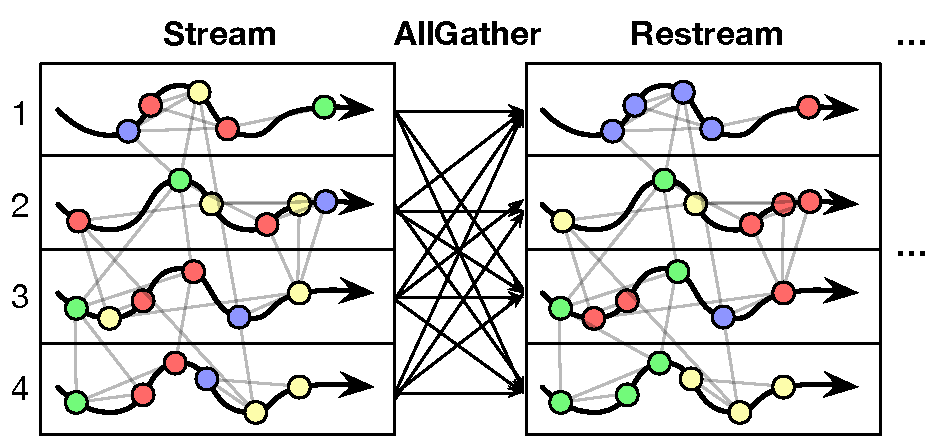
\includegraphics[width=1.0\columnwidth]{figures/restreamdiagram.pdf}
  %\caption{Partition speed of various Kronecker graphs.}
  \label{fig:coverfig}
  \caption{Parallel streaming partitioning.}
\end{figure}

\todo{Brief math for WDG}\\


\todo{pseudocode for iterative WDG}\\

% \subsection{Features}
% Our implementation can read graphs in three formats (Harwell-Boeing, Matlab, and Matrix-Market Formats).
% This allows us to read in the entire SNAP graph archive~\cite{Leskovec-data}.
% It can read in symmetric (undirected) and unsymmetric (directed) graphs.
% Once the graph is read in, we convert it from unordered triplet format to Compressed Sparse Row format, which allows us to iterate through the neighbor list of any node in linear time, as well as compute the degree of any node in constant time.

% Once we have our graph stored as a matrix in CSR form, we can perform a simulation of streaming $k-$partitioning.
% First we generate the traversal order of the graph (a random vertex order, which we generate using a Knuth Shuffle).
% We maintain a data structure that contains the assignment of every assigned vertex to its partition.
% Thus, for a given vertex, we can compute the number of edges from that vertex to each partition by iterating over each edge incident to the vertex.
% We also maintain a running total of vertices in each partition.
This process lets us compute the FENNEL algorithm in $O(|E|)=O(nnz(A))$ time.